\documentclass[twocolumn]{aastex631}
\usepackage{subfigure}
\graphicspath{{./pictures/}}

\begin{document} 

   \title{Constraint result to the self-interacting dark matter particle mass from the
   observational data}

   \author{Yixuan Zhu}\affiliation{Department of Astronomy, Beijing Normal University,
   Beijing 100875, China}
 
   \begin{abstract}

   \end{abstract}
   
   \keywords{}

\section{Introduction}\label{sec:1}

   The standard Λ-Cold Dark Matter (ΛCDM) model has been successful in 
   explaining the accelerated expansion of the Universe (\cite{Riess_1998,Perlmutter_1999}), 
   from the cosmic microwave background (CMB) anisotropies (\cite{Bennett_1996}) to 
   the measurement of baryon acoustic oscillations (BAO; \cite{Eisenstein_2005}). 
   However, there are also many alternative models that have been proposed to describe 
   the phenomenon, such as the canonical ``quintessence" scalar field theories 
   (\cite{PhysRevD.37.3406, WETTERICH1988668,PhysRevLett.80.1582}),
   non-canonical ``k-essence" theories (\cite{PhysRevLett.85.4438, PhysRevD.63.103510})
   and the modified gravity models (see, e.g., \cite{CLIFTON20121} for a review).

   It has been shown that dark matter self-interaction could contribute 
   to the accelerated expansion without dark energy component (\cite{PhysRevD.64.063501, Balakin_2003}). 
   According to the Boltzmann formalism, the disequilibrium between dark matter particle
   creation and annihilation processes would creat an effective source term 
   making negative pressure just like the dark energy. \cite{Basilakos_2009}
   investigated the analytical solutions for the simple interacting dark matter (IDM) 
   model, and find that the effective annihilation term is much smaller than the
   results given by the general methods. The gravitational matter creation model (\cite{Lima_2008})
   is mathematically equivalent to one case of the IDM models (\cite{Basilakos_2009}).

   In this paper, we use the newly revised data from $H(z)$, supernovae Ia 
   and baryon acoustic oscillation by using the Markov chain Monte
   Carlo (MCMC) method. The constraint result gives an upper limit for the 
   linear ratio between the dark matter annihilation cross section $\langle\sigma v\rangle$
   and the dark matter particle mass $M_{\chi}$ about $9\times10^{-15} \;\text{cm}^{3}\text{s}^{-1}\text{GeV}^{-1}$. 

   The paper is arranged as follows: In Sec.\ref{sec:2}, we review the basic equations in the IDM model,
   in Sec.\ref{sec:3}, we introduce the observational datasets used in this analysis, in Sec.\ref{sec:4}, 
   we give the constraint results of the IDM model and compare our results with 
   other relevant dark matter constraints, and finally we conclude in Sec.\ref{sec:5}.

\section{The basic equations in the IDM model}\label{sec:2}

   We assume that the total density of the cosmic fluid obeys
   the collisional Boltzmann equation (\cite{Kolb:1990vq})
   \begin{equation}
      \dot{\rho}+3H\rho+\kappa\rho^2-2\Psi=0,
      \label{eq:1}
   \end{equation}
   where $\rho$ is the total energy-density of the cosmic fluid,
   containing dark matter, baryons, and any type of exotic energy,
   $\Psi$ is the rate of creation of DM particle pairs, and the
   annihilation parameter $\kappa(\geq0)$ is given by:
   \begin{equation}
      \kappa=\frac{\langle\sigma v\rangle}{M_{\chi}},
      \label{eq:2}
   \end{equation}
   where $\sigma$ is the cross section for annihilation, $v$ is
   the mean particle velocity, and $M_{\chi}$ is the mass of the DM
   particle.
   Compared to the usual fluid equation, the effective pressure term
   is \begin{equation}
      P=\frac{\kappa\rho^2-\Psi}{3H}.
      \label{eq:3}
   \end{equation}
   When $\kappa\rho^2-\Psi<0,$ what means that the IDM particle
   creation term is larger than the annihilation item, IDM may serve
   as a negative pressure source in the global dynamics of the Universe,
   like the role of Dark Energy in the general cosmological models.

   \cite{Basilakos_2009} identified two functional forms for which
   the previous Boltzmann equation can be solved analytically.
   Refering to Appendix B in \cite{Basilakos_2009}, only one of these two is of interest
   because it provides a ``$\propto\alpha^{-3}$'' dependence of the scale factor,
   which is \begin{equation}
      \Psi(\alpha)=\alpha H(\alpha)R(\alpha)=C_1(n+3)\alpha^nH(\alpha)+\kappa C_1^2 \alpha^{2m}.
      \label{eq:4}
   \end{equation}
   And the total energy density is
   \begin{equation}
      \rho(\alpha)=C_1 \alpha^n+\frac{\alpha^{-3}F(\alpha)}{C_2-\int_1^{\alpha}x^{-3}f(x)F(x)\mathrm{d}x},
      \label{eq:5}
   \end{equation}
   where $f(\alpha)=-\kappa/[\alpha H(\alpha)],$ and the kernal function $F(\alpha)$ has
   the form \begin{equation}
      F(\alpha)=\exp\left[-2\kappa C_1\int_1^{\alpha}\frac{x^{n-1}}{H(x)}\mathrm{d}x\right].
      \label{eq:6}
   \end{equation}
   The first term of Eq.(\ref{eq:5}) is the density corresponding to the
   residual matter creation that results from a possible disequilibrium
   between the particle creation and annihilation processes, while the second
   term can be viewed as the energy density of the self-IDM particles that are
   dominated by the annihilation process.

\subsection{Model 1: relation to the ΛCDM model}

   If $n=0$, the global density evolution can be transformed as
   \begin{equation}
      \rho(\alpha)=C_1+\alpha^{-3}\frac{e^{-2\kappa C_1(t-t_0)}}{C_2+\kappa Z(t)},
      \label{eq:7}
   \end{equation}
   where $Z(t)=\int_{t_0}^t \alpha^{-3}e^{-2\kappa C_1(t'-t_0)}\mathrm{d}t'$ (\cite{Basilakos_2009}).
   Using the usual unit-less $\Omega$-like parameterization, we obtain that
   \begin{equation}
      \left(\frac{H}{H_0}\right)^2=\Omega_{1,0}+\frac{\Omega_{1,0}\Omega_{2,0}\alpha^{-3}e^{-2\kappa C_1(t-t_0)}}
      {\Omega_{1,0}+\kappa C_1\Omega_{2,0}Z(t)},
      \label{eq:8}
   \end{equation}
   where $\Omega_{1,0}=8\pi GC_1/3H_0^2$ and $\Omega_{2,0}=8\pi G/3H_0^2C_2$,
   which related to $\Omega_{\Lambda}$ and $\Omega_m$ in the $\Lambda$CDM model,
   respectively.
   From Eq.({\ref{eq:2}}), we can also give the mass of the DM particle
   related to the range of $\kappa C_1$(in the unit of Gyr${}^{-1}$)
   \begin{equation}
      M_{\chi}=\frac{3.325\times10^{-12}}{\kappa C_1}
      \frac{\langle\sigma v\rangle}{10^{-23}}h^2(1-\Omega_{2,0})\,\text{GeV},
      \label{eq:9}
   \end{equation}
   where $h\equiv H_0/[100\text{km/s/Mpc}]$.

\subsection{Model 2 : relation to the wCDM model}

   If $n\neq0$, the global density evolution is Eq.(\ref{eq:5}), and the 
   usual unit-less $\Omega$-like can be written as
   \begin{equation}
      \left(\frac{H}{H_0}\right)^2 = \Omega_{1,0} \alpha^n + 
      \frac{\Omega_{1,0} \Omega_{2,0} \alpha^{-3}F(\alpha)}
      {\Omega_{1,0} + \kappa C_1 \Omega_{2,0} \int_1^\alpha 
      \frac{F(x)}{x^4 H(x)} \mathrm{d}x},
      \label{eq:10}
   \end{equation}
   where $\Omega_{1,0}$ and $\Omega_{2,0}$ are the same defined as Eq.(\ref{eq:8}), and 
   $F(\alpha)$ is given by Eq.(\ref{eq:6}).

   Considering the limit of $\kappa \to0$, the global density evolution can be
   simplified as
   \begin{equation}
      \rho(\alpha)=C_1 a^{n}+\frac{1}{C_2} a^{-3},
      \label{eq:11}
   \end{equation}
   and Eq.(\ref{eq:10}) becomes
   \begin{equation}
      \left(\frac{H}{H_0}\right)^2=\Omega_{1,0}\alpha^{n}+\Omega_{2,0}\alpha^{-3}.
      \label{eq:12}
   \end{equation}
   The conditions $n>2$ indicates that the IDM model has an inflection point (\cite{Basilakos_2009}),
   and we define $w_{\text{IDM}}=-1-n/3$ as the equation of state (EoS) of the IDM model.
   This solution is mathematically equivalent to that of the gravitational matter 
   creation model of \cite{Lima_2008}.
   
\section{Dataset}\label{sec:3}

   To constrain the relevant IDM models (\cite{Basilakos_2009}), we use the newly revised
   observational $H(z)$ data (OHD)(\cite{PhysRevD.71.123001, Daniel.Stern_2010, 
   M.Moresco_2012, Zhang_2014, Moresco_2016, 10.1093/mnras/stx301, 10.1093/mnrasl/slv037, 
   Borghi_2022, Jiao_2023}), the Pantheon+ set of 1701 SNe Ia 
   (\cite{Scolnic_2022}), the BAO data from SDSS-IV (\cite{PhysRevD.103.083533}) and DESI DR2 
   (\cite{desicollaboration2025desidr2resultsii}).

\subsection{The observational H(z) data}

   It is widely known that the Hubble parameter $H(z)$ depends on
   the differential age as a function of redshift $z$ in the form
   \begin{equation}
      H(z)=-\frac{1}{1+z}\frac{\mathrm{d}z}{\mathrm{d}t},
      \label{eq:13}
   \end{equation}
   which provides a direct measurement on $H(z)$ based on
   $\mathrm{d}z/\mathrm{d}t$.
   OHD measurements have recently been acquired mainly employing
   cosmic chronometers (CC). The CC method is used to provide 33 observational
   data points, which are taken in the redshift range [0.07, 1.965].
   The Table \ref{tab:1} lists the OHD dataset used in this analysis.
   In this case, $\chi^2$ can be defined as
   \begin{equation}
      \chi_{\text{OHD}}^2=\sum_i\frac{(H_{\text{th}}-H_{\text{data}})^2}{\sigma_i^2}.
      \label{eq:14}
   \end{equation}

   \begin{table}
      \centering
      \begin{tabular}{ccl}
         \hline\hline
         $z$ & $H(z)$ & Reference \\
         \hline     
         0.07 & $69 \pm 19.6$ & \cite{Zhang_2014} \\
         0.09 & $69 \pm 12$ & \cite{PhysRevD.71.123001} \\
         0.12 & $68.6 \pm 26.2$ & \cite{Zhang_2014} \\
         0.17 & $83 \pm 8$ & \cite{PhysRevD.71.123001} \\
         0.179 & $75 \pm 4$ & \cite{M.Moresco_2012} \\
         0.199 & $75 \pm 5$ & \cite{M.Moresco_2012} \\
         0.2 & $72.9 \pm 29.6$ & \cite{Zhang_2014} \\
         0.27 & $77 \pm 14$ & \cite{PhysRevD.71.123001} \\
         0.28 & $88.8 \pm 36.6$ & \cite{Zhang_2014} \\
         0.352 & $83 \pm 14$ & \cite{M.Moresco_2012} \\
         0.3802 & $83 \pm 13.5$ & \cite{Moresco_2016}  \\
         0.4 & $95 \pm 17$ & \cite{PhysRevD.71.123001} \\
         0.4004 & $77 \pm 10.2$ & \cite{Moresco_2016} \\
         0.4247 & $87.1 \pm 11.2$ & \cite{Moresco_2016} \\
         0.4497 & $92.8 \pm 12.9$ & \cite{Moresco_2016} \\
         0.47 & $89 \pm 34$ & \cite{10.1093/mnras/stx301} \\
         0.4783 & $80.9 \pm 9$ & \cite{Moresco_2016} \\
         0.48 & $97 \pm 62$ & \cite{Daniel.Stern_2010} \\
         0.593 & $104 \pm 13$ & \cite{M.Moresco_2012} \\
         0.68 & $92 \pm 8$ & \cite{M.Moresco_2012} \\
         0.75 & $98.8 \pm 33.6$ & \cite{Borghi_2022} \\
         0.781 & $105 \pm 12$ & \cite{M.Moresco_2012} \\
         0.8 & $113.1 \pm 15.1$ & \cite{Jiao_2023} \\
         0.875 & $125 \pm 17$ & \cite{M.Moresco_2012} \\
         0.88 & $90 \pm 40$ & \cite{Daniel.Stern_2010} \\
         0.9 & $117 \pm 23$ & \cite{PhysRevD.71.123001} \\
         1.037 & $154 \pm 20$ & \cite{M.Moresco_2012} \\
         1.3 & $168 \pm 17$ & \cite{PhysRevD.71.123001} \\
         1.363 & $160 \pm 33.6$ & \cite{10.1093/mnrasl/slv037} \\
         1.43 & $177 \pm 18$ & \cite{PhysRevD.71.123001} \\
         1.53 & $140 \pm 14$ & \cite{PhysRevD.71.123001} \\
         1.75 & $202 \pm 40$ & \cite{PhysRevD.71.123001} \\
         1.965 & $186.5 \pm 50.4$ & \cite{10.1093/mnrasl/slv037} \\
         \hline\hline    
      \end{tabular}
      \caption{
         The OHD dataset from different reference.
      }
      \label{tab:1}
   \end{table}

\subsection{Type Ia supernovae}

   SNe Ia have long been used as ``standard candles" to give a direct
   measurement of their luminosity distance, and provides strong constraints
   on cosmological parameters. We use the latest Pantheon+ data set of 1701 
   SNe Ia samples (\cite{Scolnic_2022}), which covers the redshift range [0, 2.26].
   
   The $\chi^2$ of SNe Ia can be defined as 
   \begin{equation}
      \chi_{\text{SNe}}^2=\Delta C^{-1} \Delta^{\text{T}}-\frac{B^2}{\mathcal{C}}+\ln\left(\frac{\mathcal{C}}{2\pi}\right),
      \label{eq:15}
   \end{equation}
   where $\Delta=(\mu_{\text{th}}-\mu_{\text{data}})$, $C^{-1}$ is the inverse of the
   covariance matrix of the SNe Ia data, $B$ is the sum of $\Delta C^{-1}$ and 
   $\mathcal{C}$ is the sum of $C^{-1}$, the distance modulus is 
   $\mu=5\log_{10}(d_L/\text{Mpc})+25$, and the luminosity distance $d_L$ 
   can be given as a function of redshift $z$
   \begin{equation}
      d_L=(1+z)\int_0^z\frac{c\mathrm{d}z'}{H(z')}.
      \label{eq:16}
   \end{equation}

\subsection{Baryon acoustic oscillation}

   The Baryon acoustic oscillation (BAO) method provides a key cosmological probe
   sensitive to the cosmic expansion history with well-controlled systematics.
   We use two BAO datasets from the SDSS-IV (\cite{PhysRevD.103.083533}) and 
   DESI DR2 (\cite{desicollaboration2025desidr2resultsii}),
   which are given at Table \ref{tab:2} respectively.
   The redshift is up to 2.33 both in the SDSS and the DESI 2024 dataset.

   The $\chi^2$ function for the BAO data is defined as
   \begin{equation}
      \chi_{\text{BAO}}^2=\sum_i\frac{(D_{\text{th}}/r_{\text{d}}-D_{\text{data}}/r_{\text{d}})^2}{\sigma_i^2},
      \label{eq:17}
   \end{equation}
   where $D$ refers to $D_{\text{M}}$, $D_{\text{H}}$, or $D_{\text{V}}$, which ara given as
   \begin{eqnarray}
      D_{\text{M}}(z)&=&c\int_0^z\frac{\text{d}z'}{H(z')},\\
      D_{\text{H}}(z)&=&\frac{c}{H(z)},\\
      D_{\text{V}}(z)&=&\left[zD_{\text{M}}^2(z)D_{\text{H}}(z)\right]^{1/3},
      \label{eq:18-20}
   \end{eqnarray}
   and $r_{\text{d}}$ is the sound horizon at the drag epoch, which is given as
   \begin{equation}
      r_{\text{d}}=\int_{z_{\text{drag}}}^{\infty}\frac{c_s(z')\text{d}z'}{H(z')},
      \label{eq:21}
   \end{equation}
   where $c_s$ is the sound speed prior to recombination.

   Mathematically, the solution of Eq.(\ref{eq:8}) will encounter the singularity
   at the upper limit of the redshift $z_{\max}$ (see Appendix), and the cross 
   parameter $r_{\text{d}}h$ is used to give the constraints.

   \begin{table*}
      \centering
      \begin{tabular}{l|cccc}
         \hline\hline
         Dataset/Tracer & $z_{\text{eff}}$ & $D_{\text{V}}/r_{\text{d}}$ & 
         $D_{\text{M}}/r_{\text{d}}$ & $D_{\text{H}}/r_{\text{d}}$ \\
         \hline
         \textbf{SDSS-IV} \\
         MGS & 0.15 & $4.51 \pm 0.14$ & --- & --- \\
         BOSS galaxy & 0.38 & --- & $10.27 \pm 0.15$ & $24.89 \pm 0.58$ \\
         BOSS galaxy & 0.51 & --- & $13.38 \pm 0.18$ & $22.43 \pm 0.48$ \\
         eBOSS LRG & 0.70 & --- & $17.65 \pm 0.30$ & $19.78 \pm 0.46$ \\
         eBOSS ELG & 0.85 & --- & $19.5 \pm 1.0$ & $19.6 \pm 2.1$ \\
         eBOSS quasar& 1.48 & --- & $30.21 \pm 0.79$ & $13.23 \pm 0.47$ \\
         Ly$\alpha$-Ly$\alpha$ & 2.33 & --- & $37.6 \pm 1.9$ & $8.93 \pm 0.28$ \\
         Ly$\alpha$-quasar & 2.33 & --- & $37.3 \pm 1.7$ & $9.08 \pm 0.34$ \\
         \hline\hline
         \textbf{DESI DR2} \\ 
         BGS & 0.295 & $7.942 \pm 0.075$  & --- & --- \\
         LRG1 & 0.510 & $12.720 \pm 0.099$ & $13.588 \pm 0.167$ & $21.863 \pm 0.425$ \\
         LRG2 & 0.706 & $16.050 \pm 0.110$ & $17.351 \pm 0.177$ & $19.455 \pm 0.330$ \\
         LRG3+ELG1 & 0.934 & $19.721 \pm 0.091$ & $21.576 \pm 0.152$ & $17.641 \pm 0.193$ \\
         ELG2 & 1.321 & $24.252 \pm 0.174$ & $27.601 \pm 0.318$ & $14.176 \pm 0.221$ \\
         QSO & 1.484 & $26.055 \pm 0.398$ & $30.512 \pm 0.760$ & $12.817 \pm 0.516$ \\
         Ly$\alpha$ & 2.330 & $31.267 \pm 0.256$ & $38.988 \pm 0.531$ & $8.632 \pm 0.101$ \\
         \hline
         LRG3 & 0.922 & $19.656 \pm 0.105$ & $21.648 \pm 0.178$ & $17.577 \pm 0.213$ \\
         ELG1 & 0.955 & $20.008 \pm 0.183$ & $21.707 \pm 0.335$ & $17.803 \pm 0.297$ \\    
         \hline\hline
      \end{tabular}
      \caption{
         The BAO+RSD measurements dataset from SDSS-IV and DESI DR2.
      }
      \label{tab:2}
   \end{table*}

\section{Constraint results and discussion}\label{sec:4}

\subsection{Constraint results to the IDM model}

   We use the Markov chain Monte Carlo (MCMC) method based 
   on the opening package \texttt{emcee} to give a global constraints
   to the free parameters $\Omega_{2,0}$ and $\log_{10}(\kappa C_1)$ in 
   Model 1 and $n$ in Model 2.
   The prior range set for free parameters are given at Table \ref{tab:3}.

   \begin{table}
      \centering
      \begin{tabular}{lll}
         \hline\hline
         parameter & initial & prior \\
         \hline
         $\Omega_{2,0}$ & 0.3 & $\mathcal{U}[0.0,1.0]$ \\
         $\log_{10}(\kappa C_1/$Gyr${}^{-1})$ & --- & $\mathcal{U}[-10,0]$ \\
         $n$ & 0 & $\mathcal{U}[-5,5]$ \\
         \hline
         $H_0$[km/(s$\cdot$Mpc)] & 70 & $\mathcal{U}[60,80]$ \\
         $r_{\text{d}}h$[Mpc] & 100 & $\mathcal{U}[50,150]$ \\
         \hline
      \end{tabular}
      \caption{
         Parameters and priors used in analysis. 
         All of the priors are flat in the ranges given. 
         The $\log_{10}(\kappa C_1)$ does not have a predicted value, 
         and the initial value of each chain is selected randomly uniformly
         within the prior range.
      }
      \label{tab:3}
   \end{table}

   The Eq.(\ref{eq:8}) convergant to the flat ΛCDM model as
   $\log_{10}(\kappa C_1)\to-\infty$, thus the constraints
   could only give the upper limit of what, and we use the
   95\% quantiles to determine the upper bounds of the parameters. 
   The constraint results are shown in 
   Figure \ref{fig:1}-\ref{fig:2} and summarized in Table \ref{tab:4}.

   For the dataset which cannot give a constraint to $H_0$, 
   we use $h \simeq 0.7$ as the default value to calculate the 
   annihilation parameter $\kappa$.
   The constraint result to the upper limit of the annihilation parameter 
   is given in Table \ref{tab:4}, which reaches a value of $\kappa = 9.07 \times 10^{-16}$ cm${}^3$/(s$\cdot$GeV) in Model 1, 
   and $1.02 \times 10^{-13}$ cm${}^3$/(s$\cdot$GeV) in Model 2 with $\kappa\neq0$ at 95\% confidence level, respectively.

   \begin{figure*}
      \centering
      \subfigure{
         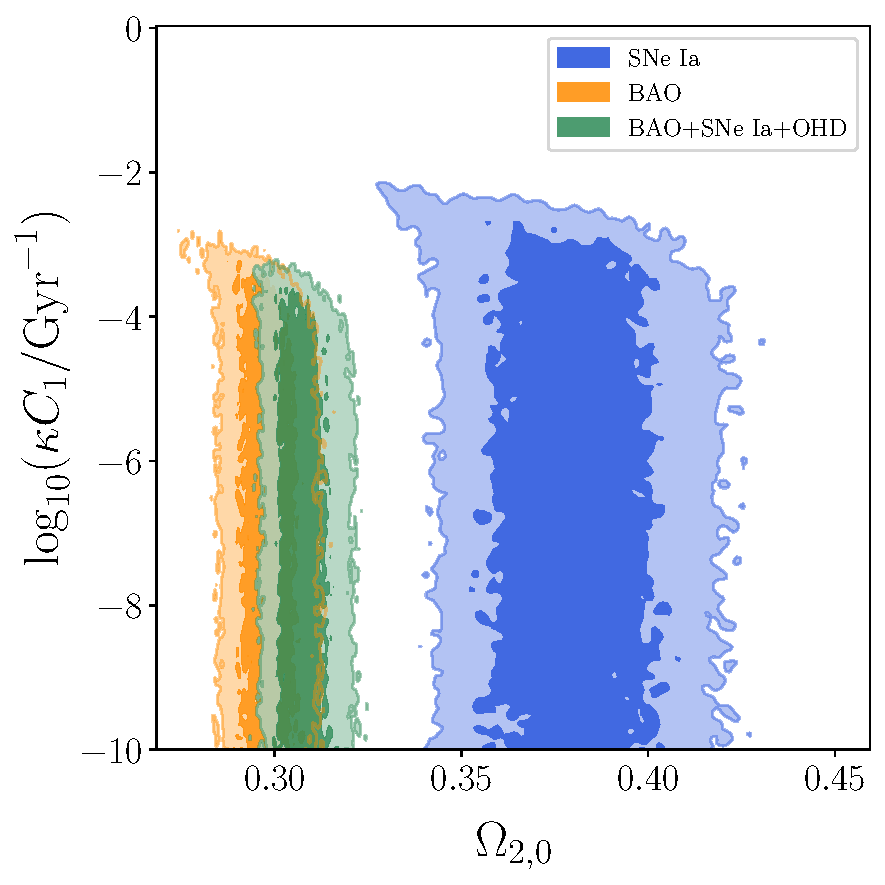
\includegraphics[width=0.45\textwidth]{model1.pdf}
      }
      \subfigure{
         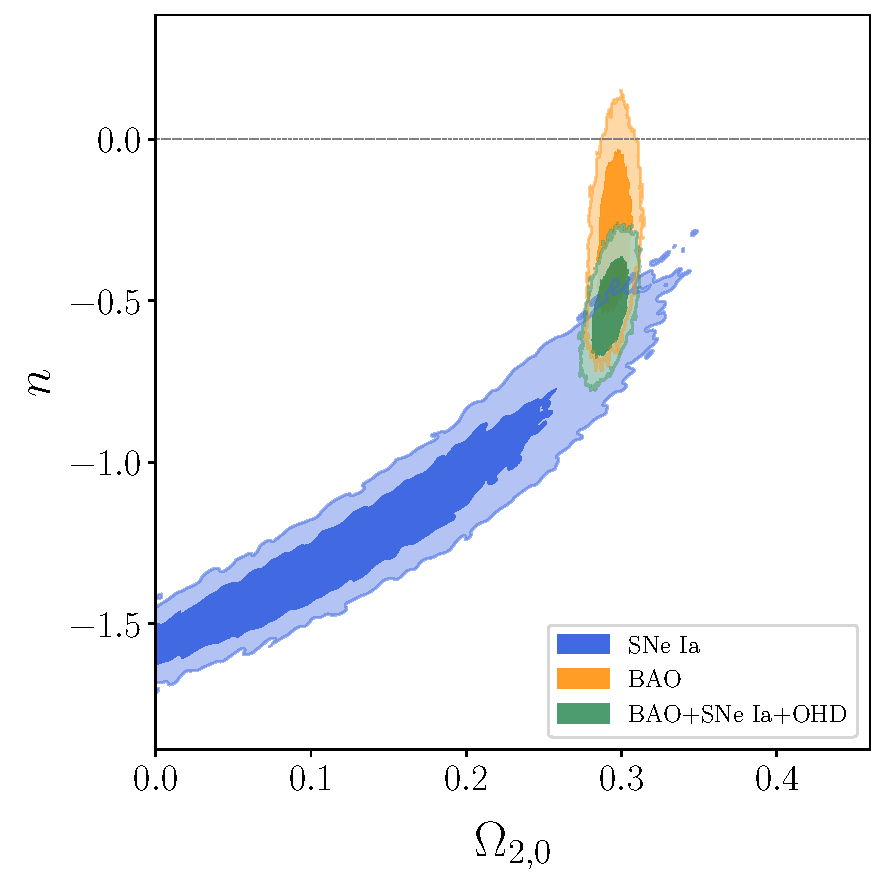
\includegraphics[width=0.45\textwidth]{model2.pdf}
      }
      \caption{
         68\% and 95\% confidence level contours for parameters in 
         IDM model. The blue, orange and green contours are the results from
         the SNe Ia dataset, the BAO dataset and the BAO + SNe Ia + OHD dataset, respectively.
         \emph{Left panel}: constraint results to $\Omega_{2,0}$ and 
         $\log_{10}(\kappa C_1/$Gyr${}^{-1})$ in Model 1. 
         \emph{Right panel}: constraint results to $\Omega_{2,0}$ and $n$ in Model 2. 
         The dashed line is $n=0$, what implies $w_{\text{IDM}}=-1$.
      }
      \label{fig:1}
   \end{figure*}
   
   \begin{figure*}
      \centering
      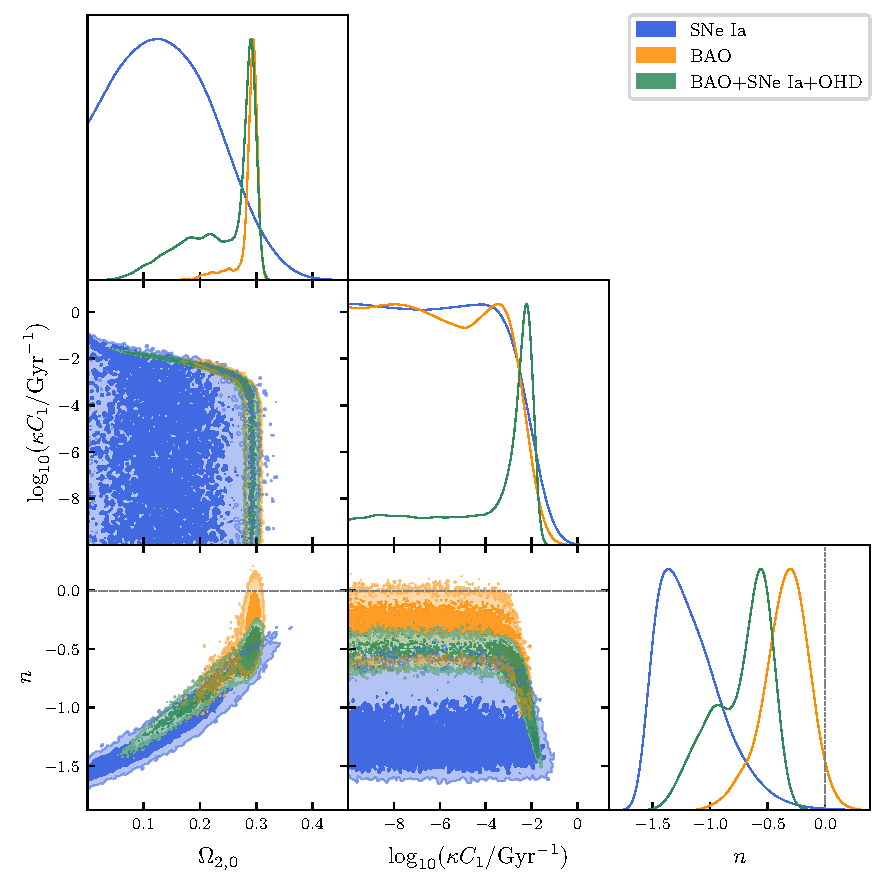
\includegraphics[width=0.9\textwidth]{model2_kneq0.pdf}
      \caption{
         Marginalized 68\% and 95\% posterior constraints on $\Omega_{2,0}$, 
         $\log_{10}(\kappa C_1/$Gyr${}^{-1})$ and $n$ in Model 2 with $\kappa\neq0$,
         from the SNe Ia dataset (blue), the BAO dataset (orange) and the 
         combination of BAO + SNe Ia + OHD dataset (green). Noted that
         the combination of BAO + SNe Ia + OHD dataset gives a two-side constraint
         to the parameter $\log_{10}(\kappa C_1/$Gyr${}^{-1})$, while we still
         use the 95\% quantile upper limit to give the constraint.
         The dashed line is $n=0$, what implies $w_{\text{IDM}}=-1$.
      }
      \label{fig:2}
   \end{figure*}

   \begin{table*}
      \centering
      \begin{tabular}{l|ccccc}
         \hline\hline
         Model/Dataset & $\Omega_{2,0}$ & $\log_{10}(\kappa C_1/$Gyr${}^{-1})$ & $10^{15}\kappa$[cm${}^3$/(s$\cdot$GeV)] & $n$ & $w_{\text{IDM}}$ \\
         \hline
         \textbf{Model 1} \\
         SNe Ia & $0.380 \pm 0.020$ & $<-3.05$ & $<8.82$ & --- & --- \\
         BAO & $0.2980 \pm 0.0070$ & $<-3.66$ & $<1.91$ & --- & --- \\
         BAO+SNe Ia+OHD & $0.3079_{-0.0067}^{+0.0051}$ & $<-3.99$ & $<0.907$ & --- & --- \\
         \hline
         \textbf{Model 2 ($\kappa=0$)} \\
         SNe Ia & $0.215_{-0.073}^{+0.10}$ & --- & --- & $-0.82_{-0.45}^{+0.29}$ & $-0.73_{-0.10}^{+0.15}$ \\
         BAO & $0.2952 \pm 0.0073$ & --- & --- & $-0.29_{-0.18}^{+0.15}$ & $-0.90_{-0.05}^{+0.06}$ \\
         BAO+SNe Ia+OHD & $0.2945 \pm 0.0075$ & --- & --- & $-0.42 \pm 0.11$ & $-0.86 \pm 0.04$ \\
         \hline
         \textbf{Model 2 ($\kappa\neq0$)} \\
         SNe Ia & $0.143_{-0.11}^{+0.067}$ & $<-2.15$ & $<50.7$ &  $-1.17_{-0.35}^{+0.17}$ & $-0.61_{-0.06}^{+0.12}$ \\
         BAO & $0.287_{-0.0022}^{+0.017}$ & $<-2.44$ & $<31.3$ & $-0.34_{-0.17}^{+0.22}$ & $-0.89_{-0.07}^{+0.06}$ \\
         BAO+SNe Ia+OHD & $0.241 \pm 0.062$ & $<-1.90$ & $<101.8$ & $-0.73_{-0.24}^{+0.33}$ & $-0.76_{-0.11}^{+0.08}$ \\
         \hline\hline
      \end{tabular}
      \caption{
         Summary table of the parameter constraints from the different datasets in
         the IDM model. Results for the parameters $\Omega_{2,0}$ and $n$ are the
         mean values with 68\% confidence level, while the $\log_{10}(\kappa C_1)$
         is the 95\% quantile upper limit.
      }
      \label{tab:4}
   \end{table*}

\subsection{The dark matter annihilation}

   We assume that the dark matter particle $\chi$ consists of Weakly Interacting Massive Particles (WIMPs),
   which can annihilate into Standard Model (SM) particles with a cross section $\langle\sigma v\rangle$, 
   and the dark matter particle in the IDM model acts as a self-annihilation process.
   
   The WIMPs assumption gives that the thermal relic abundance of dark matter requires 
   an annihilation cross section of $\langle\sigma v \rangle $ about $ 3\times 10^{-26}$ cm${}^3$/s
   to match the observed cosmological density
   (\cite{PhysRevLett.39.165,annurev:/content/journals/10.1146/annurev.ns.29.120179.001525, GONDOLO1991145}).
   Adopting this value in the IDM model, the lower limit of the dark matter particle mass can be given as
   $M_{\chi} \gtrsim 3 \times 10^{-2}$ eV in Model 1 and 
   $3 \times 10^{-4}$ eV in Model 2 with $\kappa\neq0$.

   \begin{figure*}
      \centering
      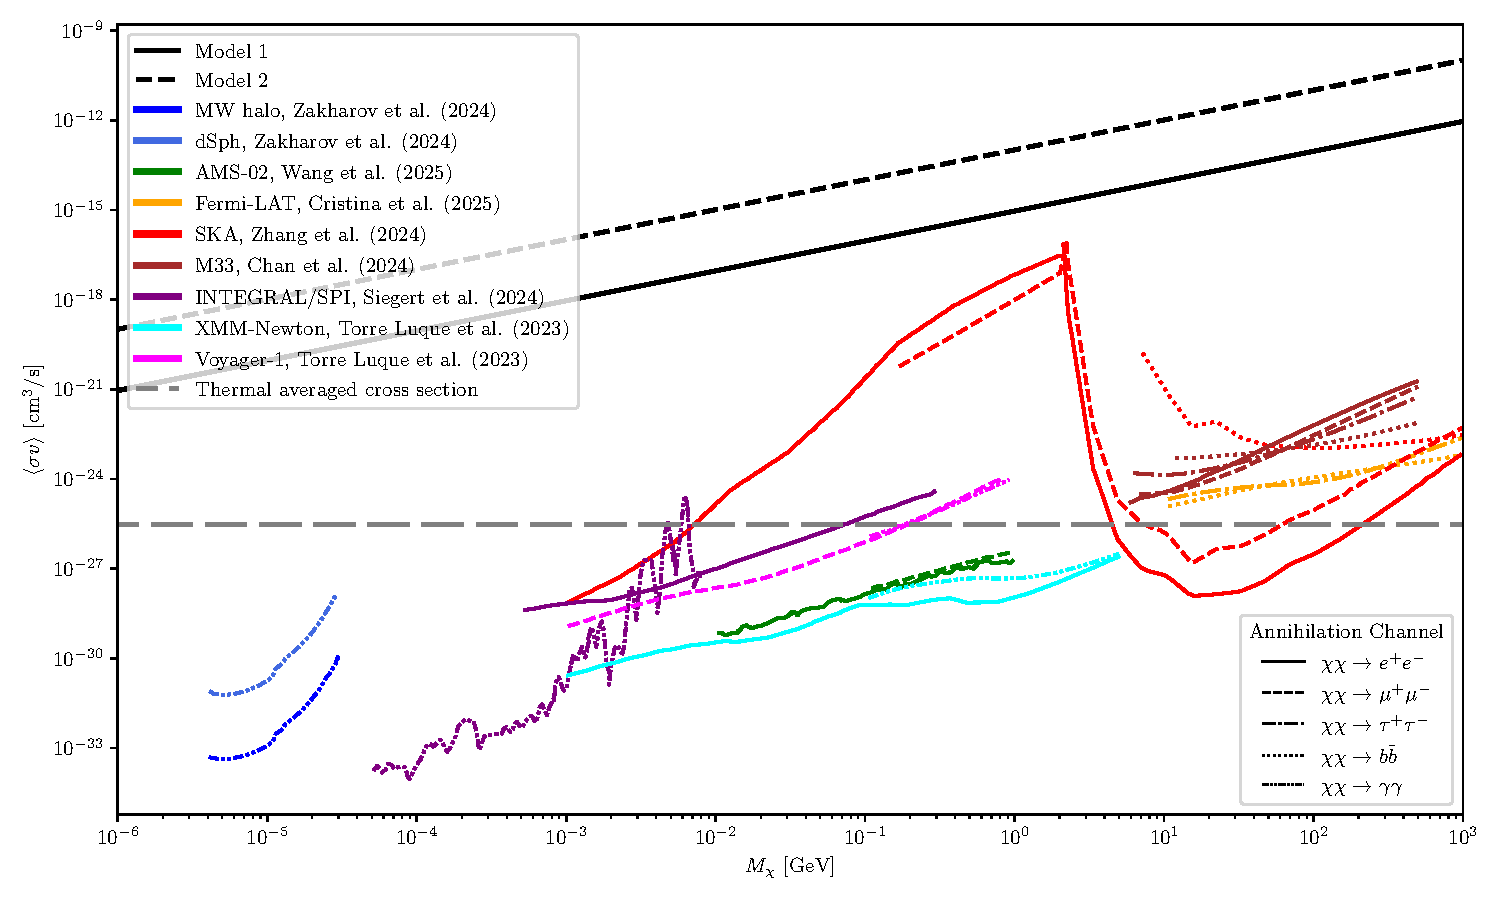
\includegraphics[width=0.9\textwidth]{dm_ann.pdf}
      \caption{The dark matter annihilation cross section $\langle\sigma v\rangle$ 
         as a function of the dark matter particle mass $M_{\chi}$ in the IDM model.
      }
      \label{fig:3}
   \end{figure*}

\section{Conclusions}\label{sec:5}

\appendix

\section{The theoretical solution of model 1}

   Apply the Eq.(\ref{eq:12}) to Eq.(\ref{eq:8}), we can get a simple nonlinear
   second-order differential equation for the redshift $z(t)$, which can
   be written as \begin{equation}
      2H_0^2\Omega_{1,0}(1+z)^2z'z''+\kappa C_1z'{}^4-5H_0^2\Omega_{1,0}(1+z)z'{}^3
      +3H_0^4\Omega_{1,0}^2(1+z)^3z'-H_0^4\Omega_{1,0}^2\kappa C_1[(z+1)^4-1]
      =H_0^4\Omega_{1,0}^2\kappa C_1,
   \end{equation}
   where the prime denotes the derivative with respect to $t$.
   The equation can be simplified as
   \begin{equation}
      2H_0^2\Omega_{1,0}y^2y'y''+\kappa C_1y'{}^4-5H_0^2\Omega_{1,0}yy'{}^3
      +3H_0^4\Omega_{1,0}^2y^3y'-H_0^4\Omega_{1,0}^2\kappa C_1y^4=0,
   \end{equation}
   where $y=z+1$, now it is a homogeneous function and we can give the
   general solution as $y=\exp{f}$ with $f$ a function of $t$, the equation
   now is \begin{equation}
      2H_0^2\Omega_{1,0}f'f''+\kappa C_1f'{}^4-3H_0^2\Omega_{1,0}f'{}^3
      +3H_0^4\Omega_{1,0}^2f'-H_0^4\Omega_{1,0}^2\kappa C_1=0.
   \end{equation}
   We use $g=f'$, which also gives $g(t)=y'/y=-H(t)$, then the equation can be written as
   \begin{equation}
      2H_0^2\Omega_{1,0}gg'+\kappa C_1g^4-3H_0^2\Omega_{1,0}g^3
      +3H_0^4\Omega_{1,0}^2g-H_0^4\Omega_{1,0}^2\kappa C_1=0.
   \end{equation}
   It can be theoretically solved and the solution has a form like
   \begin{equation}
      g(t)=\mathcal{G}\left(-\frac{t}{2H_0^2\Omega_{1,0}}+Const\right),
   \end{equation}
   where $\mathcal{G}$ is the inverse function of
   \begin{equation}
      \mathcal{F}(x)=\frac{3H_0\sqrt{\Omega_{1,0}}\mathrm{arctanh}\frac{x}{H_0\sqrt{\Omega_{1,0}}}
      -\kappa C_1\log(x^2-H_0^2\Omega_{1,0})+\kappa C_1\log(\kappa C_1x^2-3H_0^2\Omega_{1,0}x
      +H_0^2\Omega_{1,0}\kappa C_1)}{9H_0^4\Omega_{1,0}^2-4H_0^2\Omega_{1,0}(\kappa C_1)^2}.
   \end{equation}
   In this term, $\displaystyle\mathrm{arctanh}(x)\doteq \frac{1}{2}\log\left(\frac{x+1}{x-1}\right)$
   when $x<-1$, and the $Const$ is determined by the boundary condition $g(0)\to -\infty$, which is

   \begin{equation}
      Const=\mathcal{F}(-\infty)\equiv\lim_{x\to-\infty}\mathcal{F}(x)=
      \frac{\kappa C_1\ln\kappa C_1}{9H_0^4\Omega_{1,0}^2-4H_0^2\Omega_{1,0}(\kappa C_1)^2}.
   \end{equation}
   The initial time of today $t_0$ can be easily given as
   \begin{equation}
      t_0=2H_0^2\Omega_{1,0}[\mathcal{F}(-\infty)-\mathcal{F}(-H_0)],
   \end{equation}
   and the redshift $z_{\max}$ can be calculated as
   \begin{equation}
      z_{\max}=\exp\left[2H_0^2\Omega_{1,0}\int_{-\infty}^{-H_0}[\mathcal{F}(-\infty)
      -\mathcal{F}(x)]\mathrm{d}x+H_0t_0\right]-1,
   \end{equation}
   and $z_{\max}$ is also a function of $\Omega_{2,0}, \kappa C_1$ and $H_0$.
   \begin{figure}
      \centering
      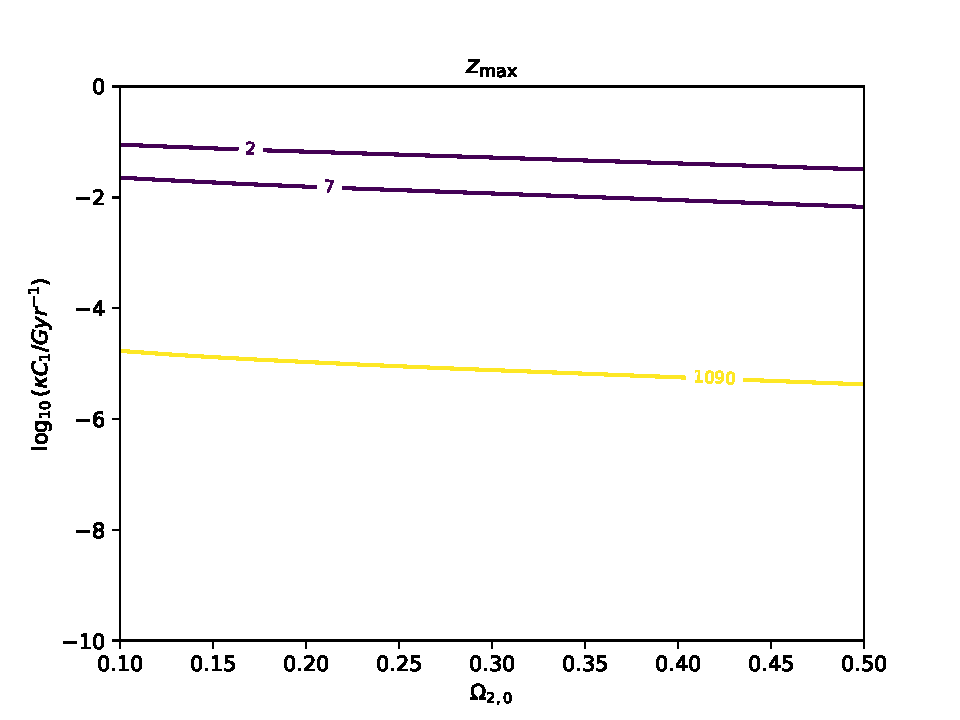
\includegraphics[width=0.7\textwidth]{zmax.pdf}
      \caption{The redshift $z_{\max}$ as $H_0=70$ km/(s$\cdot$Mpc)}
      \label{fig:3}
   \end{figure}

\bibliography{reference}
\bibliographystyle{aasjournal}

\end{document}